\documentclass[12pt,letterpaper]{article}
\usepackage{graphicx,textcomp}
\usepackage{setspace}
\usepackage{fullpage}
\usepackage{color}
\usepackage[reqno]{amsmath}
\usepackage{amsthm}
\usepackage{fancyvrb}
\usepackage{amssymb,enumerate}
\usepackage[all]{xy}
\usepackage{endnotes}
\usepackage{lscape}
\newtheorem{com}{Comment}
\usepackage{float}
\usepackage{hyperref}
\newtheorem{lem} {Lemma}
\newtheorem{prop}{Proposition}
\newtheorem{thm}{Theorem}
\newtheorem{defn}{Definition}
\newtheorem{cor}{Corollary}
\newtheorem{obs}{Observation}
\usepackage[compact]{titlesec}
\usepackage{dcolumn}
\usepackage{tikz}
\usetikzlibrary{arrows}
\usepackage{multirow}
\usepackage{xcolor}
\newcolumntype{.}{D{.}{.}{-1}}
\newcolumntype{d}[1]{D{.}{.}{#1}}
\definecolor{light-gray}{gray}{0.65}
\usepackage{url}
\usepackage{listings}
\usepackage{color}
\usepackage{indentfirst}
\usepackage{amssymb} 
\usepackage{threeparttable}
\usepackage{caption}
\usepackage{booktabs}
\usepackage{array}
\usepackage{longtable}


\definecolor{codegreen}{rgb}{0,0.6,0}
\definecolor{codegray}{rgb}{0.5,0.5,0.5}
\definecolor{codepurple}{rgb}{0.58,0,0.82}
\definecolor{backcolour}{rgb}{0.95,0.95,0.92}

\lstdefinestyle{mystyle}{
	backgroundcolor=\color{backcolour},   
	commentstyle=\color{codegreen},
	keywordstyle=\color{magenta},
	numberstyle=\tiny\color{codegray},
	stringstyle=\color{codepurple},
	basicstyle=\footnotesize,
	breakatwhitespace=false,         
	breaklines=true,                 
	captionpos=b,                    
	keepspaces=true,                 
	numbers=left,                    
	numbersep=5pt,                  
	showspaces=false,                
	showstringspaces=false,
	showtabs=false,                  
	tabsize=2
}
\lstset{style=mystyle}
\newcommand{\Sref}[1]{Section~\ref{#1}}
\newtheorem{hyp}{Hypothesis}

\usepackage[american]{babel}
\usepackage{csquotes}

\usepackage[
style=apa,
backend=biber
]{biblatex}

\addbibresource{rep.bib}

\title{Replication Project}
\date{Descriptive and Substantive Representation in Congress \\ Evidence from 80,000 Congressional Inquiries\\ April 1, 2026}
\author{Shelly Veal-Upham\\
	25337422}

\begin{document}
	\maketitle
	\captionsetup[table]{labelformat=empty} 
	
	\section{Original Study}
	
	My replication project centers around the study "Descriptive and Substantive Representation in Congress: Evidence from 80,000 Congressional Inquiries" by Kenneth Lowande, Melinda Ritchie, and Erinn Lauterbach (2019). The study's main purpose is to explore the relationship between descriptive and substantive representation as measured by a U.S. congress members' likelihood to contact federal agencies on behalf of a group of protected legal status (women, veterans, or racial/ethnic minorities) if they share that background \parencite{lowande2019}.\\
	
	\begin{center}
		\noindent \textit{Implicit Research Question: Does descriptive representation result in substantive representation as measured by Congress members' post-legislative followup with federal agencies?} \\
		\vspace{0.2cm}
		In other terms:\\
		\vspace{0.2cm}
		\textit{Do members of Congress who share identities/experiences with citizen demographics of protected legal status inquire more frequently to federal agencies on behalf of said citizens?}\\
	\end{center}
	
	\subsection*{Methods}
	
	The authors submitted Freedom of Information Act (FOIA) requests to federal agencies and compiled 88,000 contacts from Congressional members between 2003 and 2015 (108th and 113th Congresses). Information on the demographic background of Congressmen and women was taken from CQ Press' congressional member profiles \parencite{cq_info} and used to determine whether the representative was a member of the protected groups of interest. Researchers hand-coded each contact according to whether or not the inquiry was made on behalf of a protected group in the U.S. (with strict requirements for affirmative coding such that the data are more likely to \textit{undercount} than overcount inquiries on behalf of citizens).\\
	
	Aggregating the data such that each observation became legislator-congress with columns for contacting on behalf of each protected group (1: contacted any federal agency on behalf of the protected group at least once during the congressional session, 0: did not contact any federal agencies on the protected group's behalf) allowed the authors to examine the direct relationship (using OLS models) between a member of congress' demographic background and the demographics of the constituents they represent.\\
	
	The researchers controlled for a variety of confounders, including representative DW-NOMINATE scores (an ideology scale ranging from -1 (extremely liberal) to +1 (extremely conservative)), district demographics (such as \% population White vs Nonwhite or Tausanovitch-Warshaw scale of ideology (also with negative scores mapping to liberal ideologies)), and congressional chamber and session.\\
	
	This study builds on the literature by examining inquiries made directly to federal agencies, something largely unobserved in the research and free from the political pressures of the other representative decisions congress members make (i.e. voting for or sponsoring a particular bill, making speeches). As such, the design allows the researchers direct access to the (they argue) true behavioral differences of representatives with differing backgrounds/identities.\\
	
	Further, including military service as a factor in their analysis and veterans as a group of protected legal status expands the literature from strictly focusing on identity as "descriptive" representation to including shared experiences. This allows the findings to support theories posited surrounding the connection between identity and shared experience as well as descriptive and substantive representation.\\
	
	\subsection*{Findings and Limitations}
	
	For each of the protected groups and the shared identity/background of legislators, the researchers found significant difference in substantive representation. That is, female legislators were more likely to contact federal agencies on behalf of women, veteran legislators were more likely to contact federal agencies on behalf of veterans, etc. \\
	
	Still, they stress that the study is a descriptive one, restricted to the particular congress people employed at the time, and the relationships uncovered should be interpreted as correlational more than causational. Further, contacting federal agencies on behalf of protected groups is only one of a myriad of potential ways to measure substantive representation. Arguments could be made for alternative explanations for a representative's tendency to contact federal agencies or not, or for alternative measures of substantive representation. As such, the results are not considered conclusive, but indicative of a tie between descriptive and substantive representation.\\
	
	\newpage
	
	\vspace{.25cm}
	\subsection*{Variables}
	
	The authors include an index with a variety of modifications on their models, including expanded use of controlling variables, but their final models (which obtain the same results as the index models) include the following variables:\\
	
\begin{table}[ht]
	\centering
	\begin{tabular}{r p{3.5cm} p{10cm}}
		\toprule
		& Variable & Description \\ 
		\midrule
		& vet.all.d & dichotomous, 1 if member contacted on behalf of veterans at least once \\ 
		& vet.10.12.d & dichotomous, 1 if member contacted on behalf of veterans at least once in 110-112 Congress and complete agency coverage \\ 
		 & fem.all.d & dichotomous, 1 if member contacted on behalf of women at least once \\ 
		 & race.ni.d & dichotomous, 1 if member contacted on behalf of
		racial/ethnic minorities at least once \\ 
		& race.ni.12.d & dichotomous, 1 if member contacted on behalf of racial/ethnic minorities at least once in 110-112 Congress and complete agency coverage \\
		\addlinespace[0.8em]
		\hline
		 & vets.exp & numeric, veteran-related expenditures in district \\ 
		 & chamber & factor, Chamber \\ 
		 & dwnom1 & continuous, Commonspace DWNOMINATE score \\ 
		& cong & numeric, Congress number \\ 
		 & tw.ideo.mean & mean constituent ideology from Tausanovitch and Warshaw \\ 
		 & white.pop & percent white population from American Community Survey \\ 
		\addlinespace[0.8em]
		\hline
		 & female & dichotomous, 1 if female legislator \\ 
		 & vet.any & dichotomous, 1 if military service background legislator \\ 
		 & vet.mainbranch & dichotomous, 1 if military service background legislator who served in something other than only reserves/national guard \\ 
		& nonwhite & dichotomous, 1 if racial/ethnic minority background legislator \\ 
		\bottomrule
	\end{tabular}
\end{table}

They utilized the following code for their own functions for cutting the data to delegations with mixed representation ("split delegations") on the identity of interest as well as ensuring standard errors of models are robust to clustering by legislator ID:\\

\newpage

	\lstinputlisting[language = R, firstline=729, lastline=758]{dataverse_files/replication.R}
	
	\newpage
	
	\section{Descriptive Data}
	
	The authors included a few figures made from the descriptive data (number of representatives with the background/identity of interest, vs. demographic indicators of their constituents). First, the overall trends in representative demography:\\
	
	\begin{figure}[h!]
		\caption*{\textbf{Figure 1: Descriptive Representation in Congress}}\label{fig1}
		\centering
		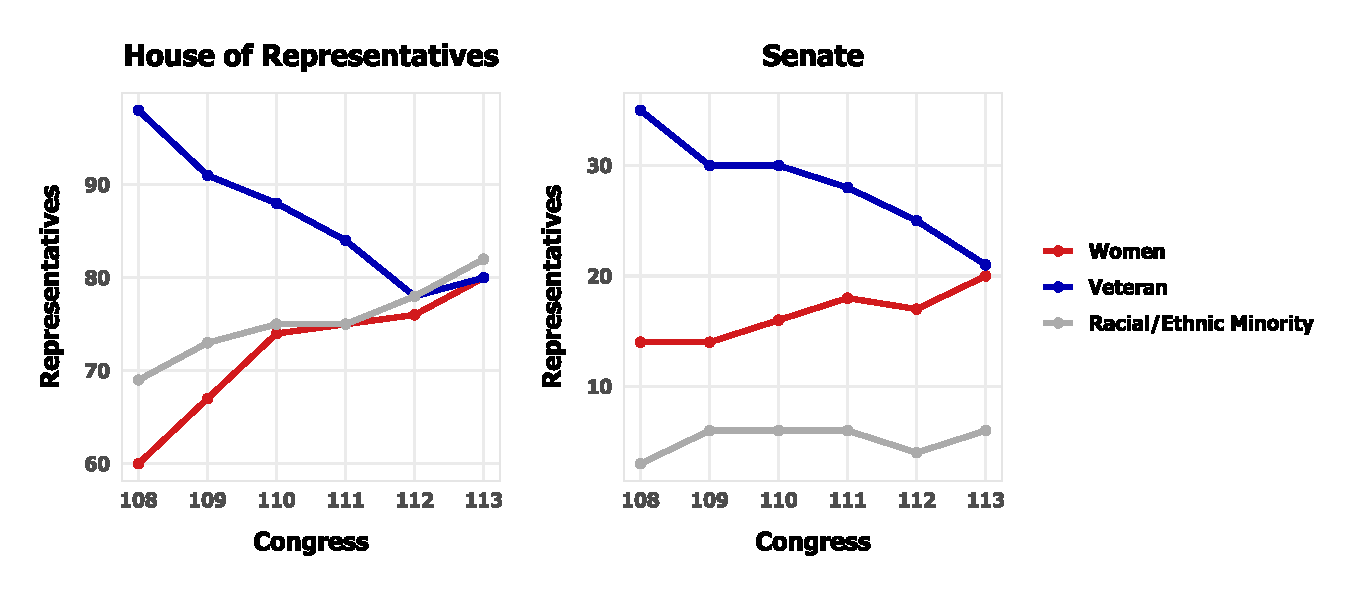
\includegraphics[width=1\textwidth]{representation.pdf}
	\end{figure}
	
	My replication code:\\
		\lstinputlisting[language = R, firstline=76, lastline=90]{dataverse_files/replication.R}
	\newpage
	Next, the article shows maps depicting constituent vs representative demography by group of legally protected status:\\
	
	\begin{figure}[h!]
		\caption*{\textbf{Figure 2.1: Descriptive Representation of Veterans}}\label{fig2.1}
		\centering
		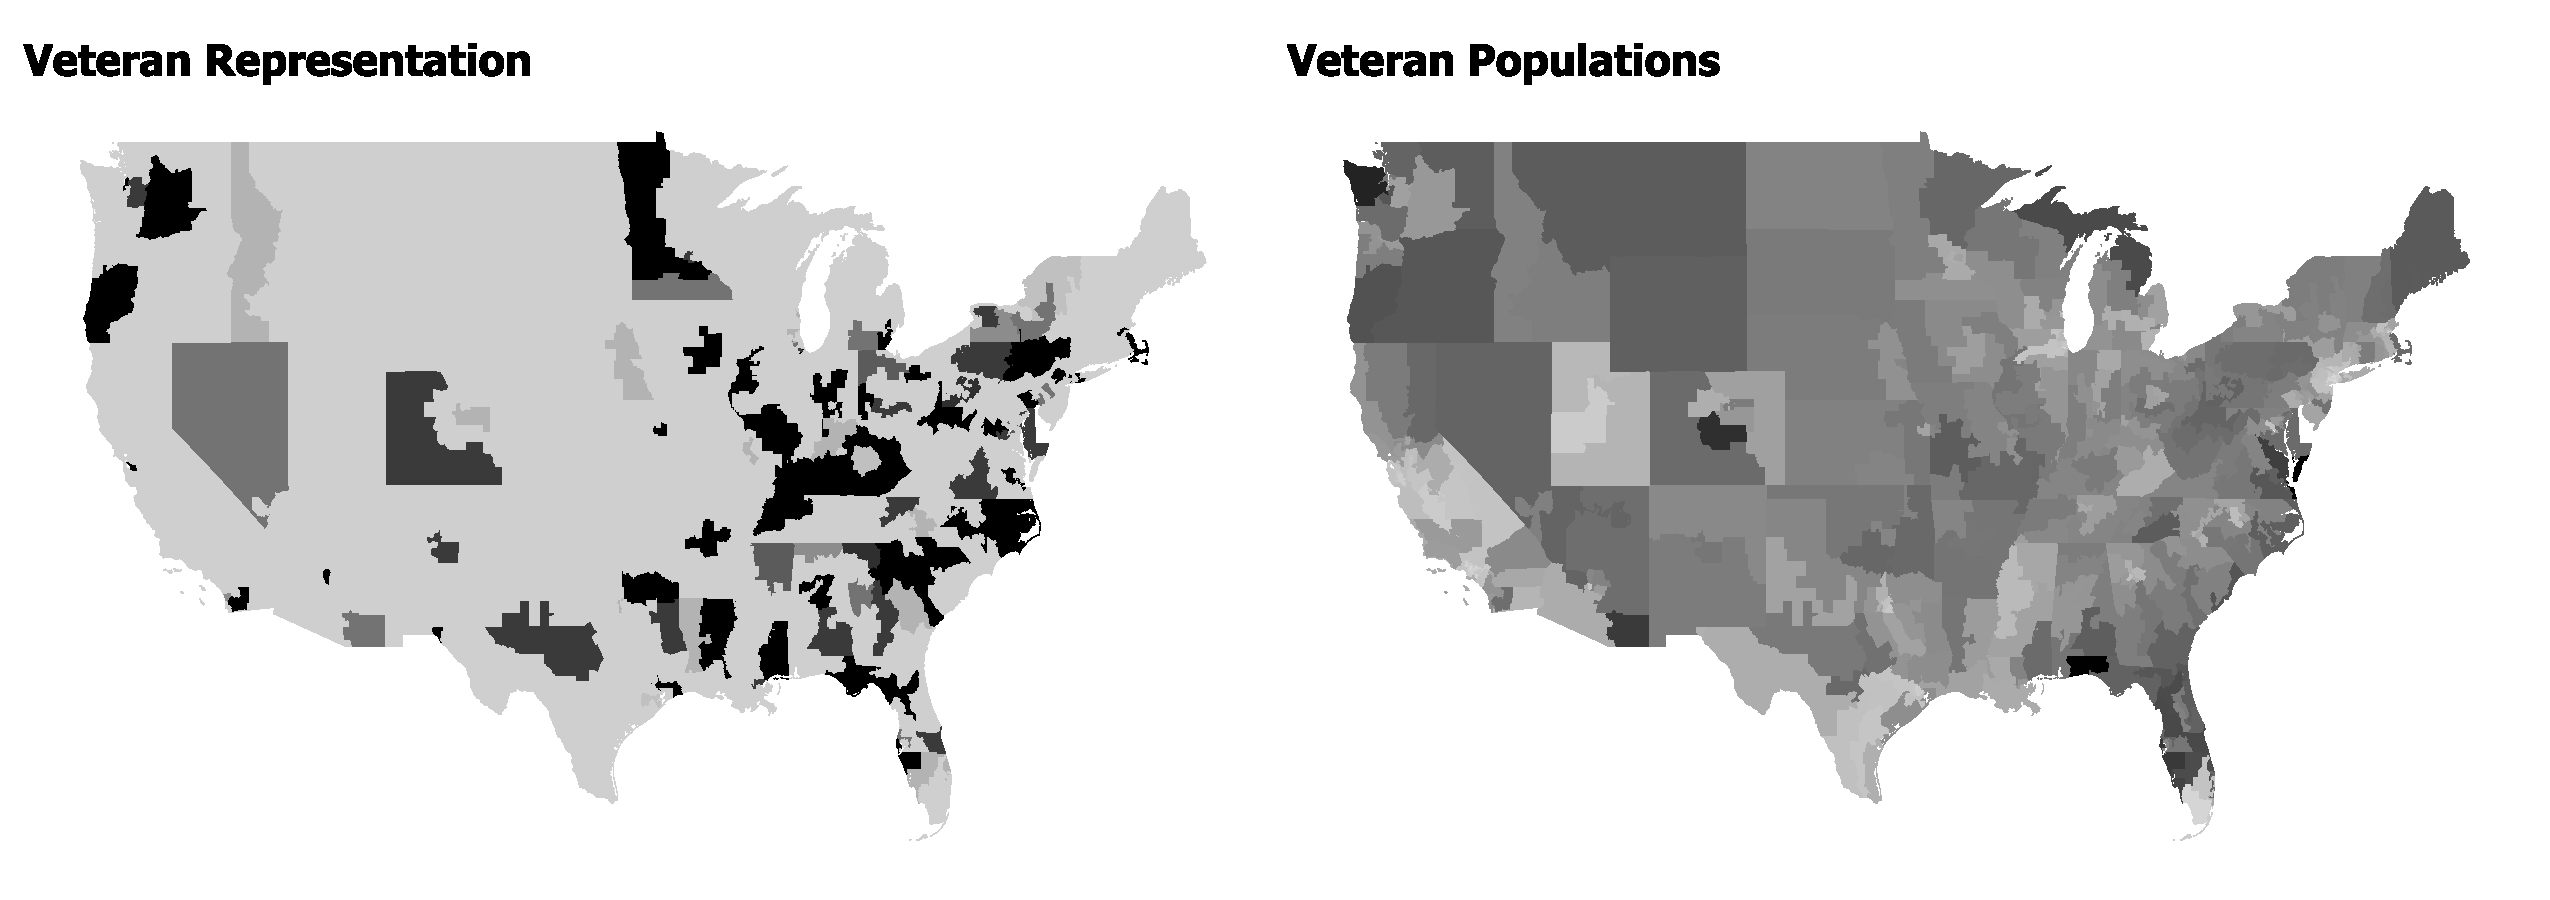
\includegraphics[width=1\textwidth]{vet_maps.pdf}
			\begin{minipage}{0.8\textwidth}
			\smallskip
			\small
			\textit{Note:}  Plots indicate proportion of legislators with military service from the 108-111th Congresses, and of the population who are veterans; darker shades indicate higher values.
		\end{minipage}
	\end{figure}
	
	\begin{figure}[h!]
		\caption*{\textbf{Figure 2.2: Descriptive Representation of Women}}\label{fig2.2}
		\centering
		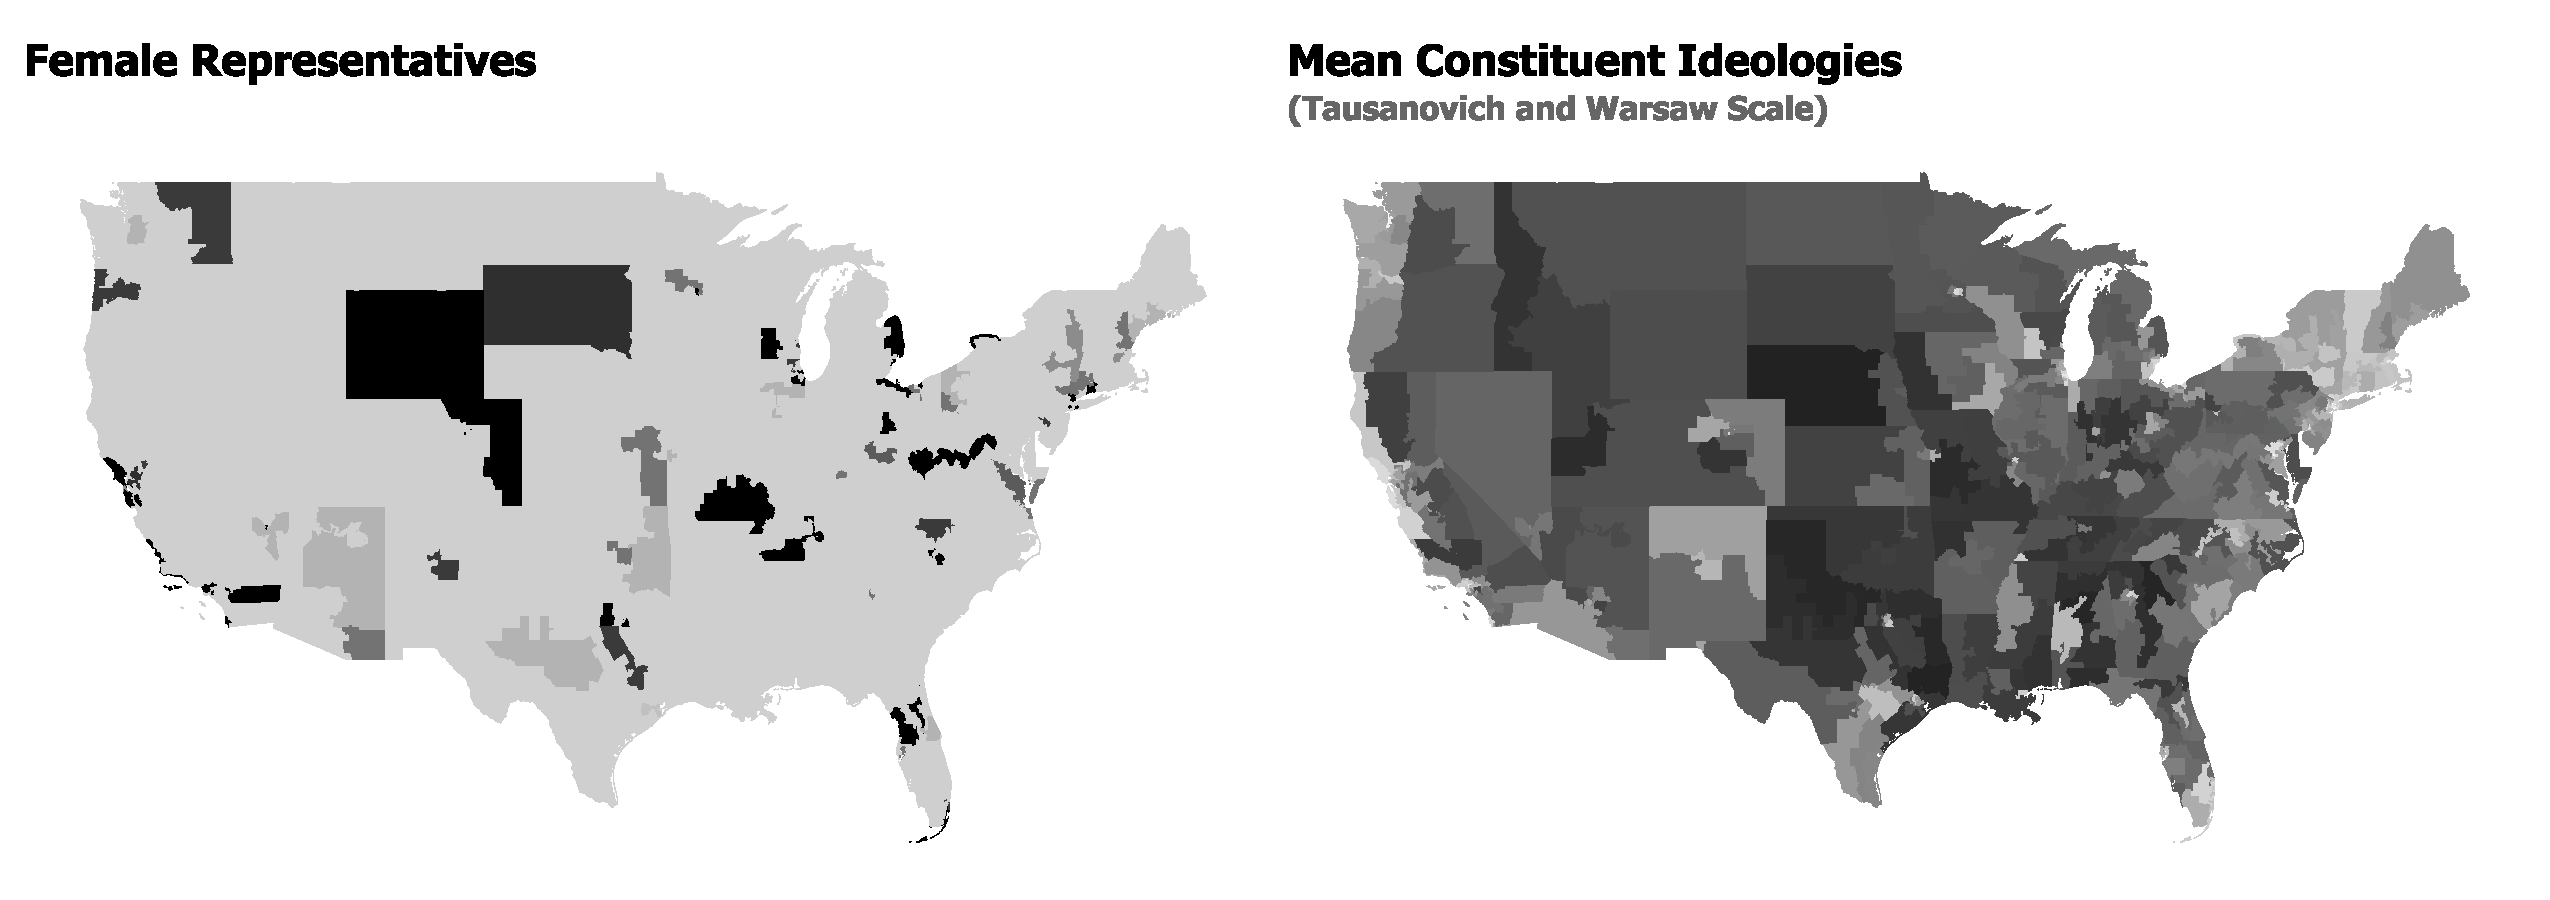
\includegraphics[width=1\textwidth]{women_maps.pdf}
			\begin{minipage}{0.8\textwidth}
			\smallskip
			\small
			\textit{Note:}  Plots indicate proportion of female legislators serving from the 108-111th Congresses, and the ideology of each district, according to Tausanovitch and Warshaw (2013); darker shades indicate higher values.
			\end{minipage}
	\end{figure}
	\newpage
	\begin{figure}[h!]
		\caption*{\textbf{Figure 2.3: Descriptive Representation of Racial/Ethnic Minorities}}\label{fig2.3}
		\centering
		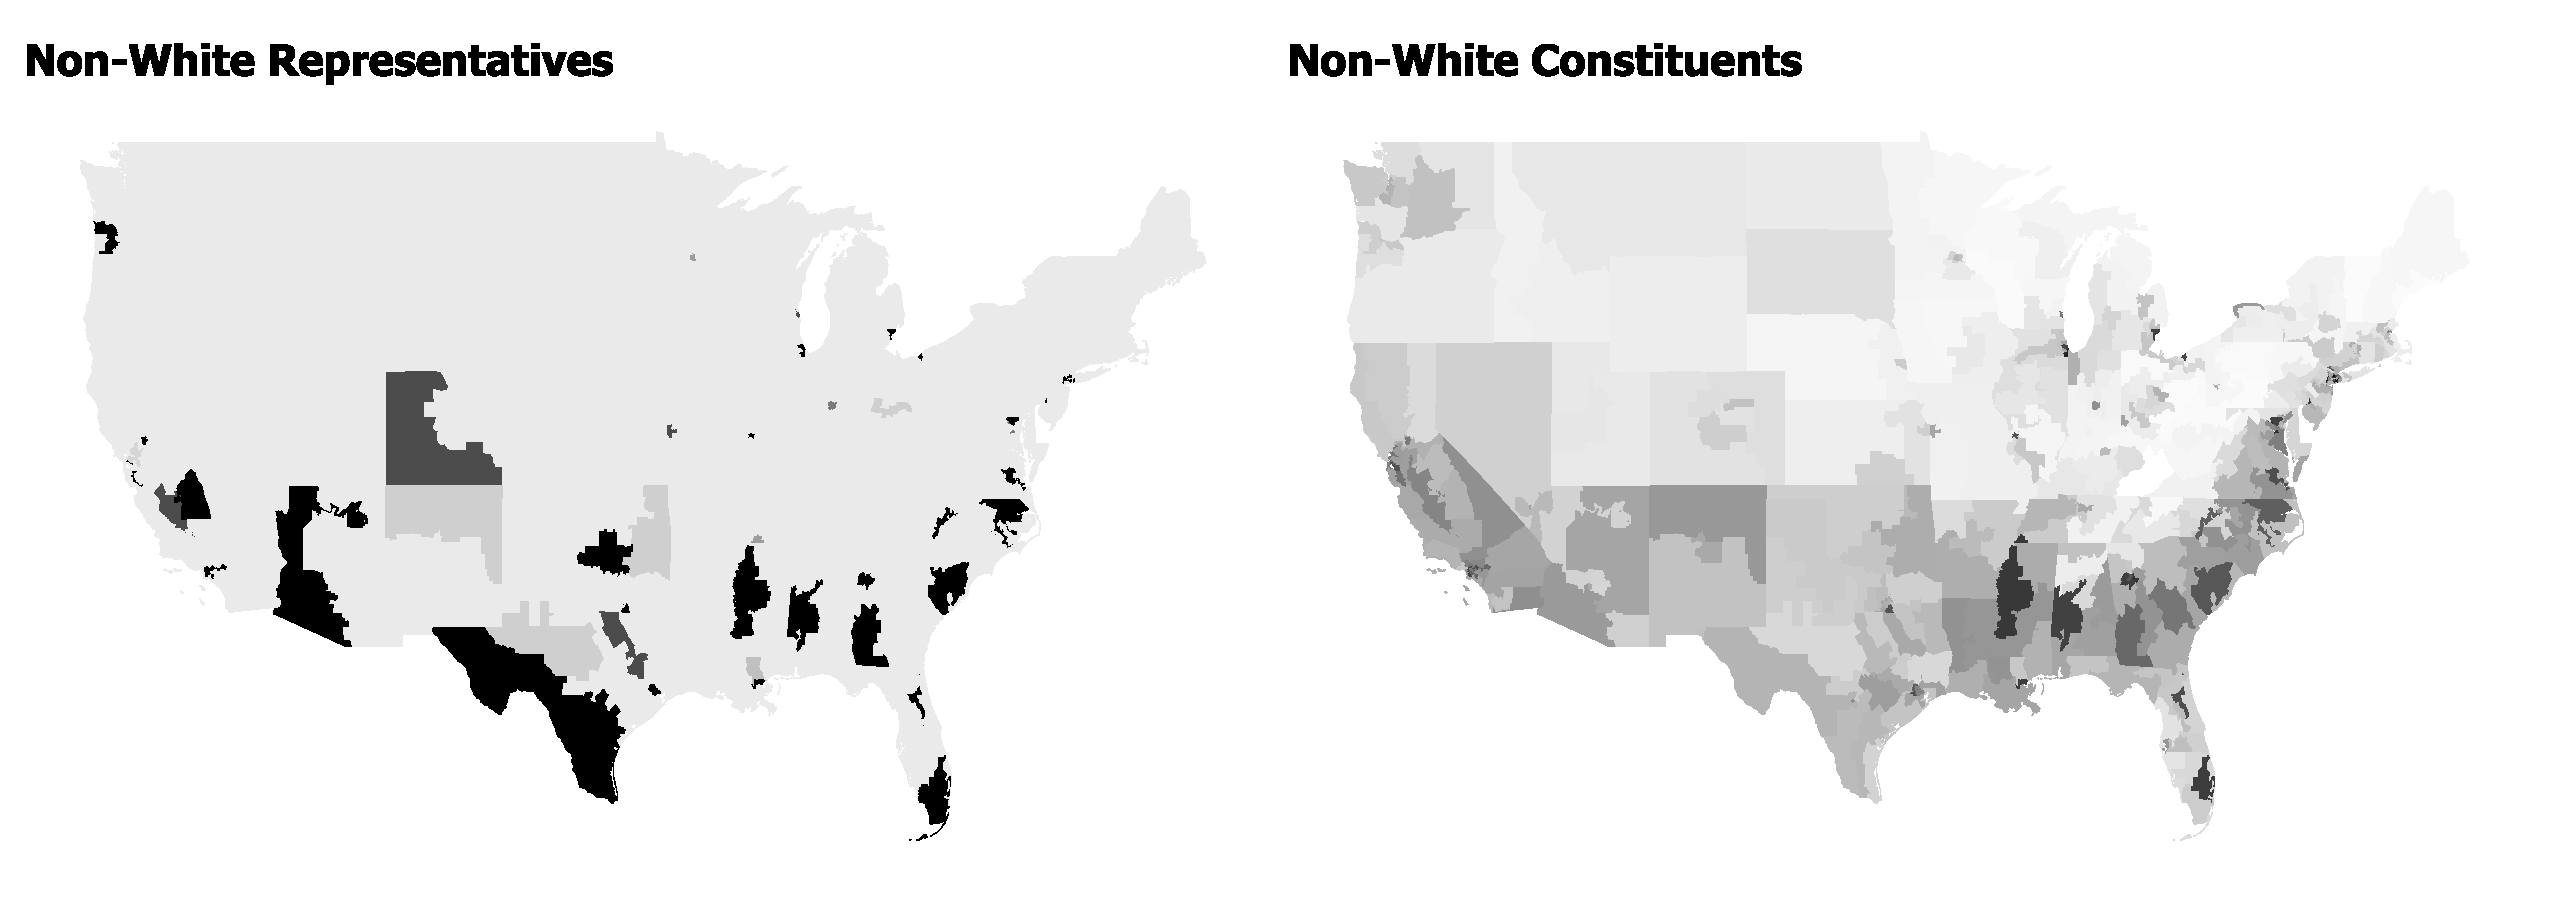
\includegraphics[width=1\textwidth]{minority_maps.pdf}
		\begin{minipage}{0.8\textwidth}
			\smallskip
			\small
			\textit{Note:}  Plots indicate proportion of legislators with racial/ethnic minority background serving from the 108-111th Congresses, and the non-white population of each district; darker shades indicate higher values.
		\end{minipage}
	\end{figure}
	
	My replication code for all maps is longer (see my \texttt{replication.R} file), but here's the code for the first map plot (first line is organizing legislator identity by geography):\\
	\lstinputlisting[language = R, firstline=99, lastline=99]{dataverse_files/replication.R}
	\lstinputlisting[language = R, firstline=106, lastline=116]{dataverse_files/replication.R}
	
	
	\section{Original Model}
	
	\subsection{Veterans}
	
	To identify whether legislators with military service backgrounds inquire on behalf of veterans more frequently than do others in Congress, the authors ran the following t-tests and compiled their mean estimates per sample group into a table I replicated in Table 2.\\
	
	\lstinputlisting[language = R, firstline=183, lastline=188]{dataverse_files/replication.R}
	
	\begin{table}[ht]
		\begin{threeparttable}
		\centering
		\caption{\textbf{Table 2: Representation Differences across Members with Military Service}}
		\label{tab2}
		\begin{tabular}{@{\extracolsep{10pt}}l@{\hspace{1.5cm}}ccc}
			\hline
			\textbf{Any Veteran} & \textbf{Nonveterans} & \textbf{Veterans} & \textbf{Difference (95 \% CI)} \\ 
			\hline
			All Legislators & 0.25 & 0.31 & +0.06 [0.1, 0.01] \\ 
			(n = 2194) &&& \\
			Split-Senate Delegations & 0.44 & 0.60 & +0.16 [0.31, 0.01] \\ 
			(n = 170) &&& \\
			\textbf{Excluding Reservists} & \textbf{Nonveterans} & \textbf{Veterans} & \textbf{Difference (95 \% CI)} \\ 
			All Legislators & 0.25 & 0.34 & +0.09 [0.15, 0.04] \\ 
			(n = 2194) &&& \\
			Split-Senate Delegations & 0.43 & 0.65 & +0.22 [0.41, 0.04] \\ 
			(n = 110) &&& \\
			\hline
		\end{tabular}
			\begin{tablenotes}[flushleft]\small
			\item \textit{Note:} Dependent variable is a dichotomous indicator of intervention on behalf of veterans in the agencies in Table 1; the unit of analysis is legislator- congress; means and difference of means are by subgroup; Split-Senate delegations are those with one member with military service.
		\end{tablenotes}
	\end{threeparttable}
	\end{table}
	
	A snippet of my replication code is here (for full code see my \texttt{replication.R} file):\\
	
	\lstinputlisting[language = R, firstline=201, lastline=207]{dataverse_files/replication.R}
	
	The authors' full models to compare whether legislators with military background (any vs. excluding reservists) are shown in Table 3. As with all replicated tables, all displayed constants are significant to at least the p<0.05 level. Below is their code for modeling. They used their custom \texttt{cl()} function mentioned above to ensure standard errors robust to their clustering.\\
	
	\lstinputlisting[language = R, firstline=216, lastline=231]{dataverse_files/replication.R}

\begin{table}[ht]
	\centering
	\begin{threeparttable}
		\caption{\textbf{Table 3: Military Service and Veterans Representation}}
		\label{tab3}
		\begin{tabular}{l@{\hspace{3cm}}cccc} 
			\hline 
			\hline
			& \multicolumn{4}{c}{\textbf{Dependent Variable:}} \\ 
			\cline{2-5} 
			& \multicolumn{2}{c}{\textbf{All Contact}} &  \multicolumn{2}{c}{\textbf{110th - 112th Cong.}}\\ 
			\cmidrule(lr){2-3} 
			\cmidrule(lr){4-5}
			& (1) & (2) & (3) & (4)\\ 
			\hline \\[-1.8ex] 
			Veteran (Any) & 0.029 &  & 0.047 &  \\ 
			& (0.024) &  & (0.028) &  \\ 
			Veteran (Excluding Reservists) &  & 0.068 &  & 0.072 \\ 
			&  & (0.030) &  & (0.032) \\ 
			Commonspace Ideology & $-$0.016 & $-$0.016 & $-$0.030 & $-$0.030 \\ 
			& (0.022) & (0.022) & (0.025) & (0.025) \\ 
			ln(Veteran Expenditures) & 0.073 & 0.073 & 0.070 & 0.071 \\ 
			& (0.015) & (0.015) & (0.019) & (0.019) \\ 
			Congress Fixed Effects & $\checkmark$ & $\checkmark$ & $\checkmark$  & $\checkmark$ \\ 
			N & 2,194 & 2,194 & 1,654 & 1,654 \\ 
			Adjusted $R^2$ & 0.15 & 0.16 & 0.09 & 0.09 \\ 
			\hline 
			\hline \\[-1.8ex] 
		\end{tabular}
		\begin{tablenotes}[flushleft]\small
			\item \textit{Note:} "All Contact" is a dichotomous indicator for intervention on behalf of veterans in the agencies in Table 1; "110th-112th" is a
			subset of these congresses for the agencies with whom we have a complete record; the unit of analysis is legislator-congress; least squares
			coefficients with standard errors are clustered by legislator in parentheses; all models control for chamber; Congress intercepts are omitted
			for readability.
		\end{tablenotes}
		\end{threeparttable}
	\end{table}
	
	For my replication table, I made minor edits to the output of the following code (grabbing R-squared's, using stargazer to format): \\
	
		\lstinputlisting[language = R, firstline=233, lastline=242]{dataverse_files/replication.R}
	
		\subsection{Women}
	
	Conducting t-tests to identify differences in substantive representation of women based on legislator gender results in significant differences. Table 4 shows my replication of the original article's summary of t-test sample mean estimates. First, their t-tests:\\
	
			\lstinputlisting[language = R, firstline=247, lastline=249]{dataverse_files/replication.R}
			
	My replication code:\\
	
			\lstinputlisting[language = R, firstline=251, lastline=264]{dataverse_files/replication.R}
	
	\begin{table}[ht]
		\centering
		\begin{threeparttable}
			\caption{\textbf{Table 4: Representation Differences across Gender}}
			\label{tab4}
			\begin{tabular}{@{\extracolsep{10pt}}l@{\hspace{1.5cm}}ccc}
				\hline
				 & \textbf{Male} & \textbf{Female} & \textbf{Difference (95 \% CI)} \\ 
				\hline
				All Legislators & 0.11 & 0.23& +0.12 [0.07, 0.16] \\ 
				(n = 2194) &&& \\
				Split-Senate Delegations & 0.13 & 0.34 & +0.21 [0.02, 0.40] \\ 
				(n = 76) &&& \\
				\hline
			\end{tabular}
			\begin{tablenotes}[flushleft]\small
				\item \textit{Note:} Dependent variable is a dichotomous indicator of intervention on behalf of women in the agencies in Table 1; the unit of analysis is legislator- congress; means and difference of means are by subgroup; Split-Senate delegations are those with one female member.
			\end{tablenotes}
		\end{threeparttable}
	\end{table}
	
	Their regressions show the important contributing factors in substantive representation of women by Congress members:\\
	
			\lstinputlisting[language = R, firstline=268, lastline=275]{dataverse_files/replication.R}

	My code for replicating their summary table in Table 5 below (again, edited slightly for neat LateX compilation):\\
	
			\lstinputlisting[language = R, firstline=276, lastline=284]{dataverse_files/replication.R}

	\begin{table}[!htbp] 
		\centering 
			\begin{threeparttable}
		\caption{\textbf{Table 5: Gender and Women's Representation}} 
		\label{tab5} 
		\begin{tabular}{@{\extracolsep{20pt}}l@{\hspace{2cm}}cc} 
			\hline
			 & \textbf{(1)} & \textbf{(2)}\\ 
			\hline \\[-1.8ex] 
			Female & 0.079 & 0.083 \\ 
			& (0.020) & (0.021) \\ 
			Commonspace Ideology & $-$0.196 &  \\ 
			& (0.015) &  \\ 
			District Ideology &  & $-$0.256 \\ 
			&  & (0.024) \\ 
			Congress Fixed Effects & $\checkmark$ & $\checkmark$ \\ 
			N & 2,194 & 2,194 \\ 
			Adjusted $R^2$ & 0.21 & 0.19 \\ 
			\hline 
			\hline \\[-1.8ex] 
		\end{tabular} 
		\begin{tablenotes}[flushleft]\small
			\item \textit{Note:} Dependent variable is a dichotomous indicator for intervention on behalf of women in the agencies in Table 1; the unit of analysis is legislator-congress; least squares coefficients with standard errors are clustered by legislator in parentheses; all models control for chamber; Congress intercepts are omitted for readability.
		\end{tablenotes}
	\end{threeparttable}
	\end{table} 
	\newpage
	\subsection{Racial/Ethnic Minorities}
	
	The authors, for racial and ethnic minorities, do not report a table of comparisons between descriptive and substantive representation overall given the small sample size of split-Senate delegations. Running a basic t-test between White and Nonwhite legislators' inquiries on behalf of racial or ethnic minorities, we do see a significant difference in means (0.267 for White reps and 0.360 for Nonwhite reps, with a confidence interval ranging between -0.15 and -0.03). \\
	
			\lstinputlisting[language = R, firstline=1064, lastline=1065]{dataverse_files/replication.R}
	
	Their OLS models are detailed below:\\
	
		\lstinputlisting[language = R, firstline=292, lastline=307]{dataverse_files/replication.R}
		
	Utilizing the following code (and some edits to the output), I replicated the table of model coefficients in Table 6:\\
	
			\lstinputlisting[language = R, firstline=310, lastline=319]{dataverse_files/replication.R}

	\begin{table}[!htbp] 
		\centering 
		\begin{threeparttable}
			\caption{\textbf{Table 6: Race/Ethnicity and Minority Representation}} 
			\label{tab6} 
			\begin{tabular}{l@{\hspace{2cm}}cccc} 
				\\[-1.8ex]\hline 
				& \multicolumn{4}{c}{\textbf{Dependent Variable:}} \\ 
				\cline{2-5} 
				& \multicolumn{2}{c}{\textbf{All Contact}} &  \multicolumn{2}{c}{\textbf{110th - 112th Cong.}}\\ 
				\cmidrule(lr){2-3} 
				\cmidrule(lr){4-5}
			    & (1) & (2) & (3) & (4)\\ 
			    \hline
				Nonwhite & 0.091 & 0.060 & 0.090 & 0.078 \\ 
				& (0.034) & (0.039) & (0.037) & (0.043) \\ 
				District Ideology & $-$0.153 &  & $-$0.203 &  \\ 
				& (0.041) &  & (0.043) &  \\ 
				District \% White &  & $-$0.276 &  & $-$0.264 \\ 
				&  & (0.075) &  & (0.082) \\ 
				Congress Fixed Effects & $\checkmark$ & $\checkmark$ & $\checkmark$  & $\checkmark$ \\ 
				N & 2,194 & 2,194 & 1,654 & 1,654 \\ 
				Adjusted $R^2$ & 0.11 & 0.12 & 0.11 & 0.11 \\ 
				\hline 
				\hline \\[-1.8ex] 
			\end{tabular} 
			\begin{tablenotes}[flushleft]\small
				\item \textit{Note:} "All Contact" is a dichotomous indicator for intervention on behalf of a racial/ethnic minority in the agencies in Table 1; "110th-112th" is a subset of these congresses for the agencies with whom we have a complete record; the unit of analysis is legislator-congress; least squares coefficients with standard errors are clustered by legislator in parentheses; all models control for chamber; Congress intercepts are omitted for readability.
			\end{tablenotes}
		\end{threeparttable}
	\end{table} 
	
	\newpage
	
	\section{My Contribution}
	\subsection{Cross-Group Representation}
	Given that the intersection of identities results in a unique experience of marginalization (i.e. the experience of Black women differs from the experience of White women) \parencite{crenshaw_intersectionality}, I wanted to investigate the relationship between gender and representation of racial minorities. Since there are too few observations of members of congress with intersecting identities (female members of a racial minority), I chose to investigate the concept of solidarity. The theoretical basis for studying solidarity is the claim that people of certain minority groups experience stronger feelings of solidarity with (or empathy for) people of other minoritized identities than do members of dominant groups in both categories \parencite{hughes_tuch_gender_racial_attitudes, Dehingia2023}. Seeing whether "solidarity" appeared in this dataset, I ran an OLS regression on racial minority representation controlling for all the same controls as the previous model (Table 6), but with the congressperson's gender as a variable rather than their race.\\
	
	\lstinputlisting[language = R, firstline=326, lastline=345]{dataverse_files/replication.R}
	
	\begin{table}[!htbp] \centering 
		\caption{\textbf{Table 7: Gender and Minority Representation}}
		\label{} 
		\begin{tabular}{l@{\hspace{2cm}}cccc} 
			\\[-1.8ex]\hline 
			& \multicolumn{2}{c}{\textbf{All Contact}} &  \multicolumn{2}{c}{\textbf{110th - 112th Cong.}}\\ 
			\cmidrule(lr){2-3} 
			\cmidrule(lr){4-5}
			& (1) & (2) & (3) & (4)\\ 
			\hline
			Female & $-$0.004 & 0.007 & $-$0.003 & 0.015 \\ 
			& (0.028) & (0.028) & (0.031) & (0.031) \\ 
			District Ideology & $-$0.201$^{***}$ &  & $-$0.250$^{***}$ &  \\ 
			& (0.041) &  & (0.042) &  \\ 
			District \% White&  & $-$0.346$^{***}$ &  & $-$0.353$^{***}$ \\ 
			&  & (0.062) &  & (0.068) \\ 
			Congress Fixed Effects & $\checkmark$ & $\checkmark$ & $\checkmark$  & $\checkmark$ \\ 
			N & 2194 & 2194 & 1654 & 1654 \\ 
			Adjusted $R^2$ & 0.1 & 0.1 & 0.11 & 0.11 \\ 
			\hline 
			\hline \\[-1.8ex] 
			\textit{Note:}  & \multicolumn{4}{r}{$^{*}$p$<$0.1; $^{**}$p$<$0.05; $^{***}$p$<$0.01} \\ 
		\end{tabular} 
	\end{table} 
	
	As Table 7 shows, across all models (all contact and 110th - 112th congresses), female identity of the lawmaker had no significant relationship with their representation of racial minorities. This is reasonable given that the literature already shows mixed results on substantive measures of solidarity across identity groups \parencite{hughes_tuch_gender_racial_attitudes}. \\
	
	\newpage
	I completed a similar trial but with race/ethnicity of the legislator compared to their tendency to represent women, controlling for the same mediating factors as Table 5.\\
	
	\lstinputlisting[language = R, firstline=359, lastline=366]{dataverse_files/replication.R}
	
	\begin{table}[!htbp] \centering 
			\caption{\textbf{Table 8: Race/Ethnicity and Women's Representation}} 
			\label{} 
		\begin{tabular}{@{\extracolsep{20pt}}l@{\hspace{2cm}}cc} 
			\hline
			& \textbf{(1)} & \textbf{(2)}\\ 
			\hline \\[-1.8ex] 
			Nonwhite & 0.020 & 0.028 \\ 
			& (0.022) & (0.024) \\ 
			Commonspace Ideology & $-$0.204$^{***}$ &  \\ 
			& (0.016) &  \\ 
			District Ideology &  & $-$0.267$^{***}$ \\ 
			&  & (0.025) \\ 
			Congress Fixed Effects & $\checkmark$ & $\checkmark$ \\
			N & 2194 & 2194 \\ 
			Adjusted $R^2$ & 0.2 & 0.18 \\ 
			\hline 
			\hline \\[-1.8ex] 
			\textit{Note:}  & \multicolumn{2}{r}{$^{*}$p$<$0.1; $^{**}$p$<$0.05; $^{***}$p$<$0.01} \\ 
		\end{tabular} 
	\end{table} 

Again, we see no significant relationship between the legislator's minoritized identity (in this case race) and their propensity for contacting federal agencies on behalf of the other protected group (in this case women). As such, we conclude that this dataset provides no evidence toward the theory of "solidarity" in substantive representation of minoritized identity groups during these congresses. Note: I chose to work with specifically identity groups (race, gender) rather than include veteran status, as the literature on solidarity only provides reasonable theoretical basis for this comparison.\\
	
	\subsection*{Logit Models}

	Part of what interested me in this study is that the authors simplify representation to a series of OLS models to identify the significance of different factors in contributing to the representation of minorities. This provides a solid foundation for building more complex inferences, and given that the outcome variables of interest are binary, I was inspired to run a logistic regression on the main variables of impact to see what predictions we might be able to make (hypothetical predictions about the nature of protected group representation at this period of time, that is -- \textit{not} forecasting predictions to present circumstances).\\
	
	One thing of note in this section of my replication project is that I chose to include all potentially pertinent variables (all variables that they include in various models) combined in each logistic regression. This may be a source of dissonance between my models and theirs, and underlines the fact that I make no claims to the validity of their results based on these regressions. They are a simple experiment in the data and practice with interpreting binary outcome regressions. \\
	
	 For a logit model on the representation of veteran citizens, I ran the following logistic regression. In the table below my code, you will see the exponentiated coefficients listed with standard errors multiplied by the odds ratios to match scale. Significance is indicated for the coefficients based on the original logistic regression output, which is listed in its fomulaic format below the table.\\
	
	\lstinputlisting[language = R, firstline=377, lastline=392]{dataverse_files/replication.R}
\newpage
	\begin{table}[!htbp] \centering 
		\caption{\textbf{Odds Ratio Coefficients for Logit Model of Veteran Representation}}
		\label{} 
		\begin{threeparttable}
		\begin{tabular}{@{\extracolsep{5pt}}lcc} 
			\hline 
			\hline
			 & (1) & (2)\\ 
			\hline \\[-1.8ex] 
			Constant & 0.003 $^{***}$ & 0.003$^{***}$ \\ 
			& (0.004) & (0.01) \\ 
			111th Congress & 0.70$^{*}$ & 0.70$^{*}$ \\ 
			& (0.14) & (0.14) \\ 
			112th Congress & \textbf{0.73} & 0.72$^{***}$ \\ 
			& \textbf{(0.15)} & (0.15) \\ 
			Veteran (Any) & 1.87$^{***}$ &  \\ 
			& (0.36) &  \\ 
			Veteran (Excluding Reservists) &  & 1.60$^{**}$ \\ 
			&  & (0.34) \\ 
			ln(Veteran Expenditures) & 1.32$^{**}$ & 1.31$^{**}$ \\ 
			& (0.17) & (0.17) \\ 
			Senate & 2.07$^{**}$ & 2.12$^{***}$ \\ 
			& (0.59) & (0.62) \\ 
			\textbf{Commonspace Ideology} & \textbf{1.24} & \textbf{1.28} \\ 
			& \textbf{(0.25)} & \textbf{(0.26)} \\ 
			\hline \\[-1.8ex] 
			Observations & 1,654 & 1,654 \\ 
			Log Likelihood & $-$507.46 & $-$510.72 \\ 
			\hline 
			\hline \\[-1.8ex] 
			\textit{Note:}  & \multicolumn{2}{r}{$^{*}$p$<$0.1; $^{**}$p$<$0.05; $^{***}$p$<$0.01} \\ 
			\end{tabular} 
			\begin{tablenotes}[flushleft]\small
			\item Reference categories are 110th Congress and the House of Representatives Chamber. Model excludes legislator contact regarding casework. Significance caluclated based on non-transformed coefficients and their standard errors. Coefficients that lost significance through logit modeling in bold text.
			\end{tablenotes}
			\end{threeparttable}
	\end{table} 
	
	Log-Odds of Veteran Representation = $-5.87 + 0.73(\texttt{senate}) + 0.21(\texttt{comspace\_ideology}) - 0.36(\texttt{111th congress}) - 0.32(\texttt{112th congress}) +0.63(\texttt{vet.any}) + 0.28(\texttt{log\_vet\_exp})$\\
	
	Log-Odds of Veteran Representation = $-5.72 + 0.75(\texttt{senate}) + 0.25(\texttt{comspace\_ideology}) - 0.36(\texttt{111th congress}) - 0.32(\texttt{112th congress}) +0.47(\texttt{vet.mainbranch}) + 0.27(\texttt{log\_vet\_exp})$\\
	
	In my logistic regression of the veteran representation variables, it is of note that the variable for commonspace ideology loses its significance. This may be due to a variety of factors, including my selection of only non-casework related inquiries. Still, it indicates that over time, a representative's personal ideology score may not stably predict their substantive representation of veterans.\\
	
	Example conclusions to be drawn from these model could include:\\
	
	Holding all else constant, districts with 1 unit higher log-expenditures on veterans had representatives (of any veteran status) with about 30\% higher odds on average of contacting federal agencies on behalf of veterans (excluding casework) between 2007 and 2013. Veteran legislators (excluding non-reservists) at this time have 60\% higher odds on average of intervening than non-veteran legislators during these congresses (holding all else constant).\\
	
	I also ran a logistic regression on women's representation, controlling for all the variables that they include combined:
	
	\lstinputlisting[language = R, firstline=395, lastline=403]{dataverse_files/replication.R}
	\newpage
	\begin{table}[!htbp] \centering 
		\caption{\textbf{Odds Ratio Coefficients for Logit Model of Women's Representation}}
	\label{} 
	\begin{threeparttable}
		\begin{tabular}{lr} 
			\hline 
			\hline
			Constant & 0.02$^{***}$ \\ 
			& (0.01) \\ 
			110th Congress & 0.36$^{**}$ \\ 
			& (0.14) \\ 
			111th Congress & 0.50$^{**}$ \\ 
			& (0.17) \\ 
			112th Congress & 0.49$^{**}$ \\ 
			& (0.18) \\ 
			Female & 2.40$^{***}$ \\ 
			& (0.74) \\ 
			\textbf{District Ideology } & \textbf{1.32} \\ 
			& \textbf{(0.82)} \\ 
			Senate & 5.20$^{***}$ \\ 
			& (1.51) \\ 
			Commonspace Ideology & 0.25$^{***}$ \\ 
			& (0.12) \\
			\hline \\[-1.8ex] 
			Observations & 2,194 \\ 
			Log Likelihood & $-$248.55 \\ 
			\hline 
			\hline \\[-1.8ex] 
			\textit{Note:}  & \multicolumn{1}{r}{$^{*}$p$<$0.1; $^{**}$p$<$0.05; $^{***}$p$<$0.01} \\ 
		\end{tabular} 
		\begin{tablenotes}[flushleft]\small
		\item Reference categories are 109th Congress and the House of Representatives Chamber. Model excludes legislator contact regarding casework. Significance caluclated based on non-transformed coefficients and their standard errors. Coefficients that lost significance through logit modeling in bold text.
		\end{tablenotes}
	\end{threeparttable}
	\end{table} 
	
		Log-Odds of Women's Representation = $-3.84 + 1.65(\texttt{senate}) - 1.39(\texttt{comspace\_ideology}) - 1.02(\texttt{110th congress}) - 0.70(\texttt{111th congress}) - 0.71(\texttt{112th congress}) + 0.87(\texttt{female}) + 0.28(\texttt{tw\_ideology})$\\
	
	Example conclusions to be drawn from this model could include:\\
	
	Holding all else constant (and excluding casework), female legislators at this time had (on average) more than double the odds of contacting federal bureaucrats on behalf of women than male legislators. Districts with 0.1 points more conservative mean ideologies had representatives with an average 3\% greater odds of intervening.\\
	
	Finally, I ran a logistic regression on racial/ethnic minority representation over all congresses, excluding casework:\\
	
	\lstinputlisting[language = R, firstline=406, lastline=413]{dataverse_files/replication.R}
	
	\begin{table}[!htbp] \centering 
		\caption{\textbf{Odds Ratio Coefficients for Logit Model of Minority Representation}}
		\label{} 
		\begin{threeparttable}
			\begin{tabular}{lr} 
				\hline 
				\hline
				Constant & 0.36$^{**}$ \\ 
				& (0.15) \\ 
				\textbf{Nonwhite}& \textbf{1.37} \\ 
				& \textbf{(0.30)} \\ 
				District Ideology & 0.39$^{***}$ \\ 
				& (0.14) \\ 
				\textbf{District \% White} & \textbf{0.50} \\ 
				& \textbf{(0.25)} \\ 
				\textbf{111th Congress} & \textbf{0.99} \\ 
				& \textbf{(0.13)} \\ 
				\textbf{112th Congress} & \textbf{1.11} \\ 
				& \textbf{(0.16)} \\ 
				Senate & 5.65$^{***}$ \\ 
				& (0.86) \\ 
				\textbf{Commonspace Ideology} & \textbf{0.96} \\ 
				& \textbf{(0.21)} \\
				\hline
				Observations & 1,654 \\ 
				Log Likelihood & $-$868.25 \\
				\hline
				\hline
				\textit{Note:}  & \multicolumn{1}{r}{$^{*}$p$<$0.1; $^{**}$p$<$0.05; $^{***}$p$<$0.01} \\ 
			\end{tabular} 
			\begin{tablenotes}[flushleft]\small
				\item Reference categories are 110th Congress and the House of Representatives Chamber. Model excludes legislator contact regarding casework. Significance caluclated based on non-transformed coefficients and their standard errors. Coefficients that lost significance through logit modeling in bold text.
			\end{tablenotes}
		\end{threeparttable}
	\end{table} 
	
	Log-Odds of Racial/Ethnic Minorities' Representation = $-1.03 + 1.73(\texttt{senate}) - 0.04(\texttt{comspace\_ideology}) - 1.02(\texttt{110th congress}) - 0.70(\texttt{111th congress}) - 0.71(\texttt{112th congress}) + 0.87(\texttt{female}) - 0.69(\texttt{tw\_ideology})$
	
	The extreme loss of significance compels me not to draw any example conclusions from this model. Potential contributing factors to the loss of significance include the combined control for district ideology and district population \% White, as well as the restriction to non-casework related inquiries between 110th and 112th congresses.\\
	
	\subsection*{Visualizing Substantive Representation over Time}
	
	Finally, I thought it would be interesting to take a look at how the authors' measure of substantive representation (excluding casework) of each protected group changed over the different congresses. While all plots seem to show a (at least minor) increase over time, it's interesting to note that the overall proportion of legislators contacting federal agencies on behalf of women seems sparse in comparison to veterans or minorities. There are many potential reasons for this: perhaps the exclusion of casework had a disproportionate impact, or perhaps legislators feel less social and political pressure to advocate on behalf of women via contact with federal bureaucrats. \\
	
	Here's a snippet of my code for creating the plots -- this is only data manipulation and plotting for the 110th congress map of women's representation, but you can find the rest in my \texttt{replication.R} file:
	
	\lstinputlisting[language = R, firstline=443, lastline=449]{dataverse_files/replication.R}
	\lstinputlisting[language = R, firstline=515, lastline=528]{dataverse_files/replication.R}
	
	\newpage
	\begin{figure}[h!]
		\caption*{\textbf{Figure 3.1: Substantive Representation of Veterans Over Time}}\label{fig3.1}
		\centering
		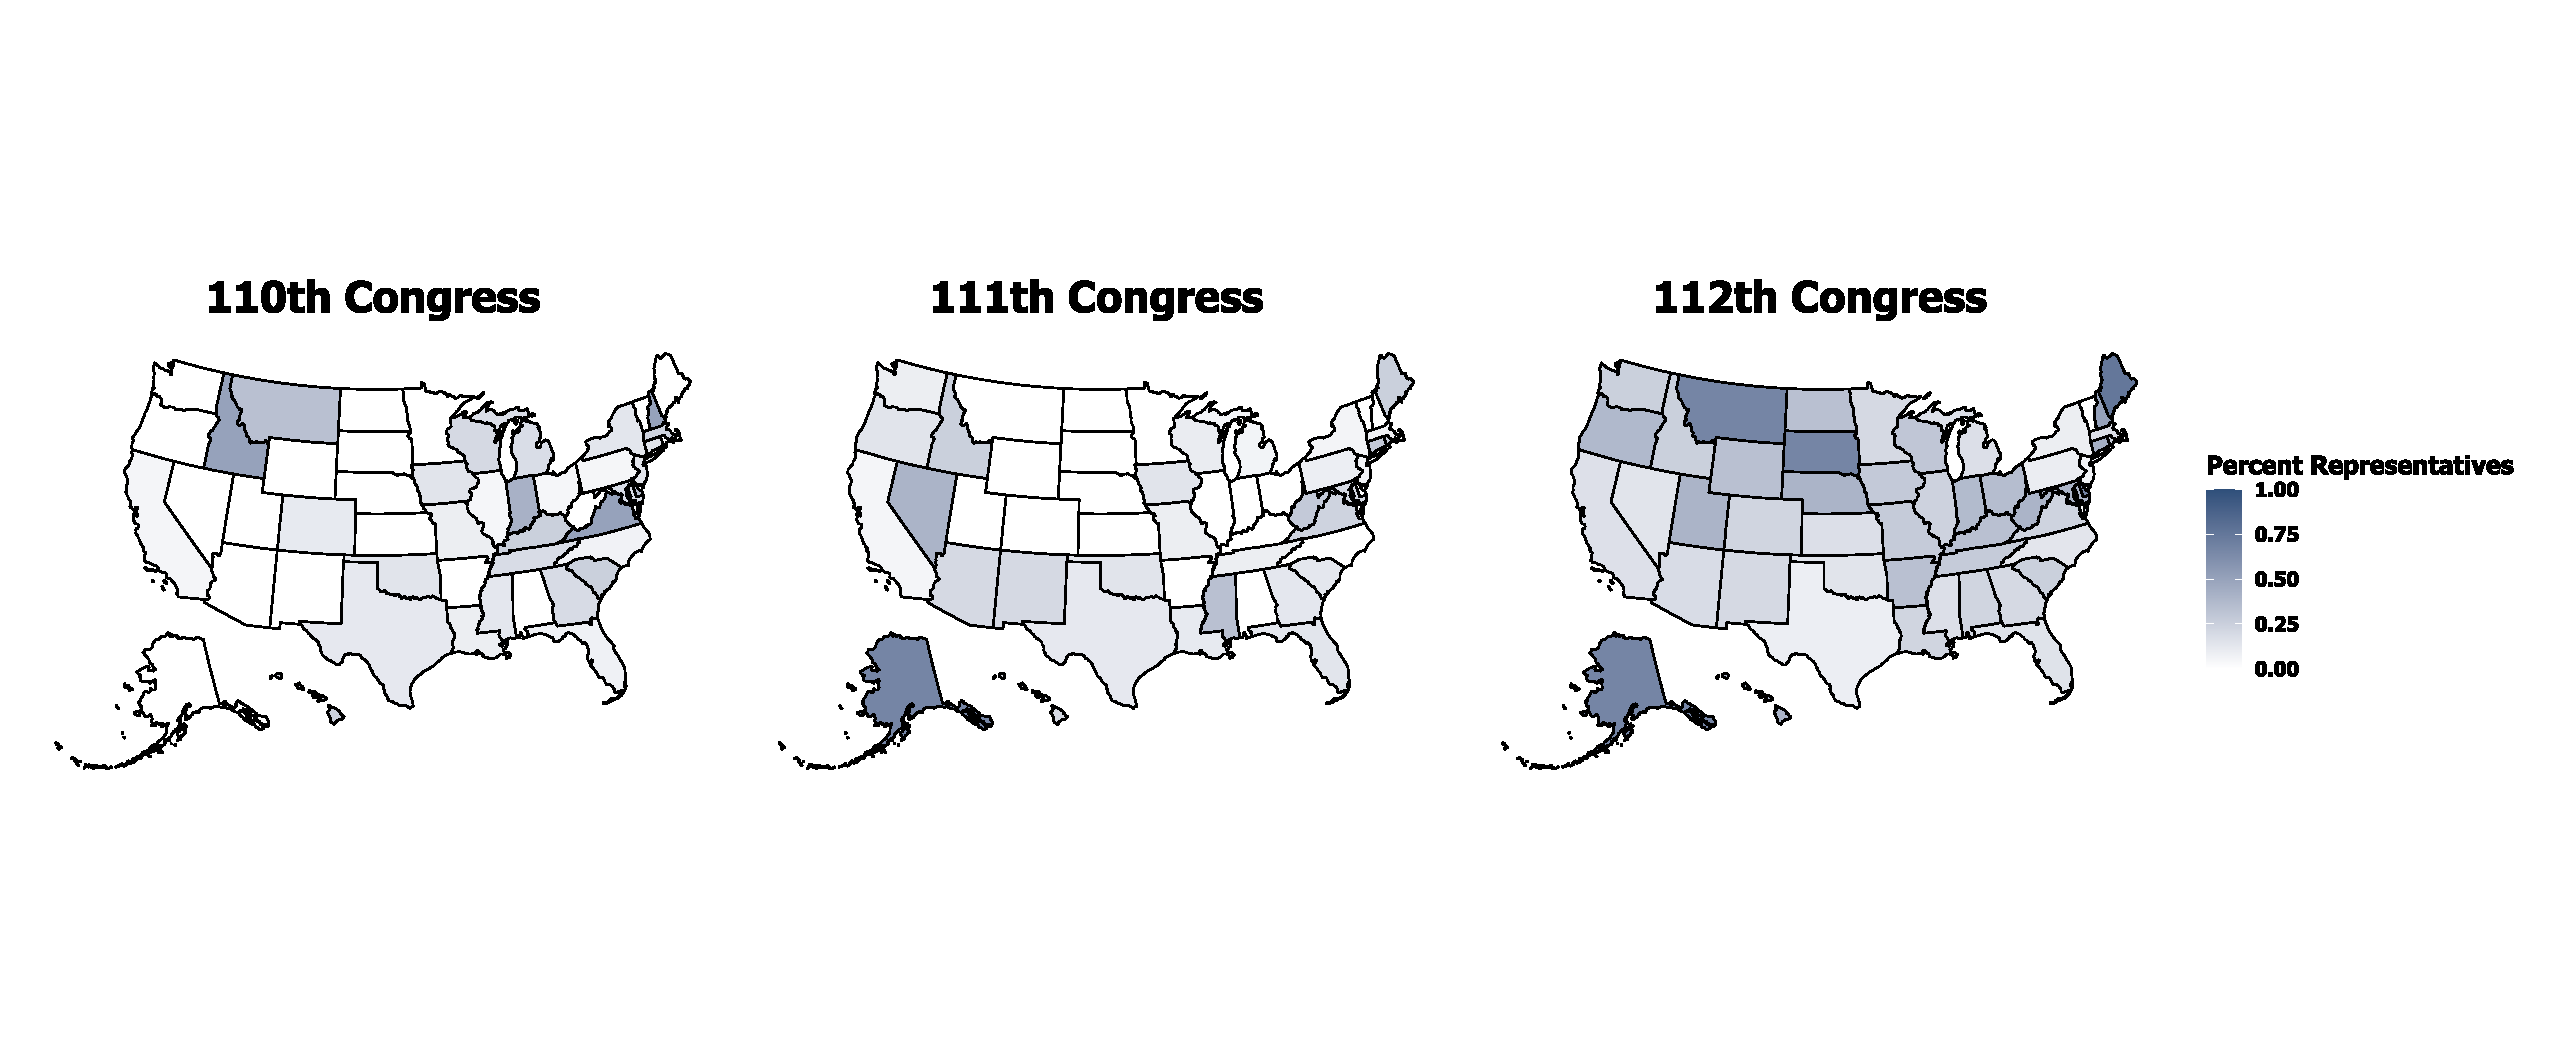
\includegraphics[width=1\textwidth]{vets_SVU_maps.pdf}
		\begin{minipage}{0.92\textwidth}
			\smallskip
			\small
			\textit{Note:}  Plots indicate proportion of legislators contacting federal agencies on behalf of veterans (excluding casework) at least once per congressional term for the 110th, 111th, and 112th Congresses. Darker shades of blue indicate higher values.
		\end{minipage}
	\end{figure}
	
	\begin{figure}[h!]
		\caption*{\textbf{Figure 3.2: Substantive Representation of Women Over Time}}\label{fig3.2}
		\centering
		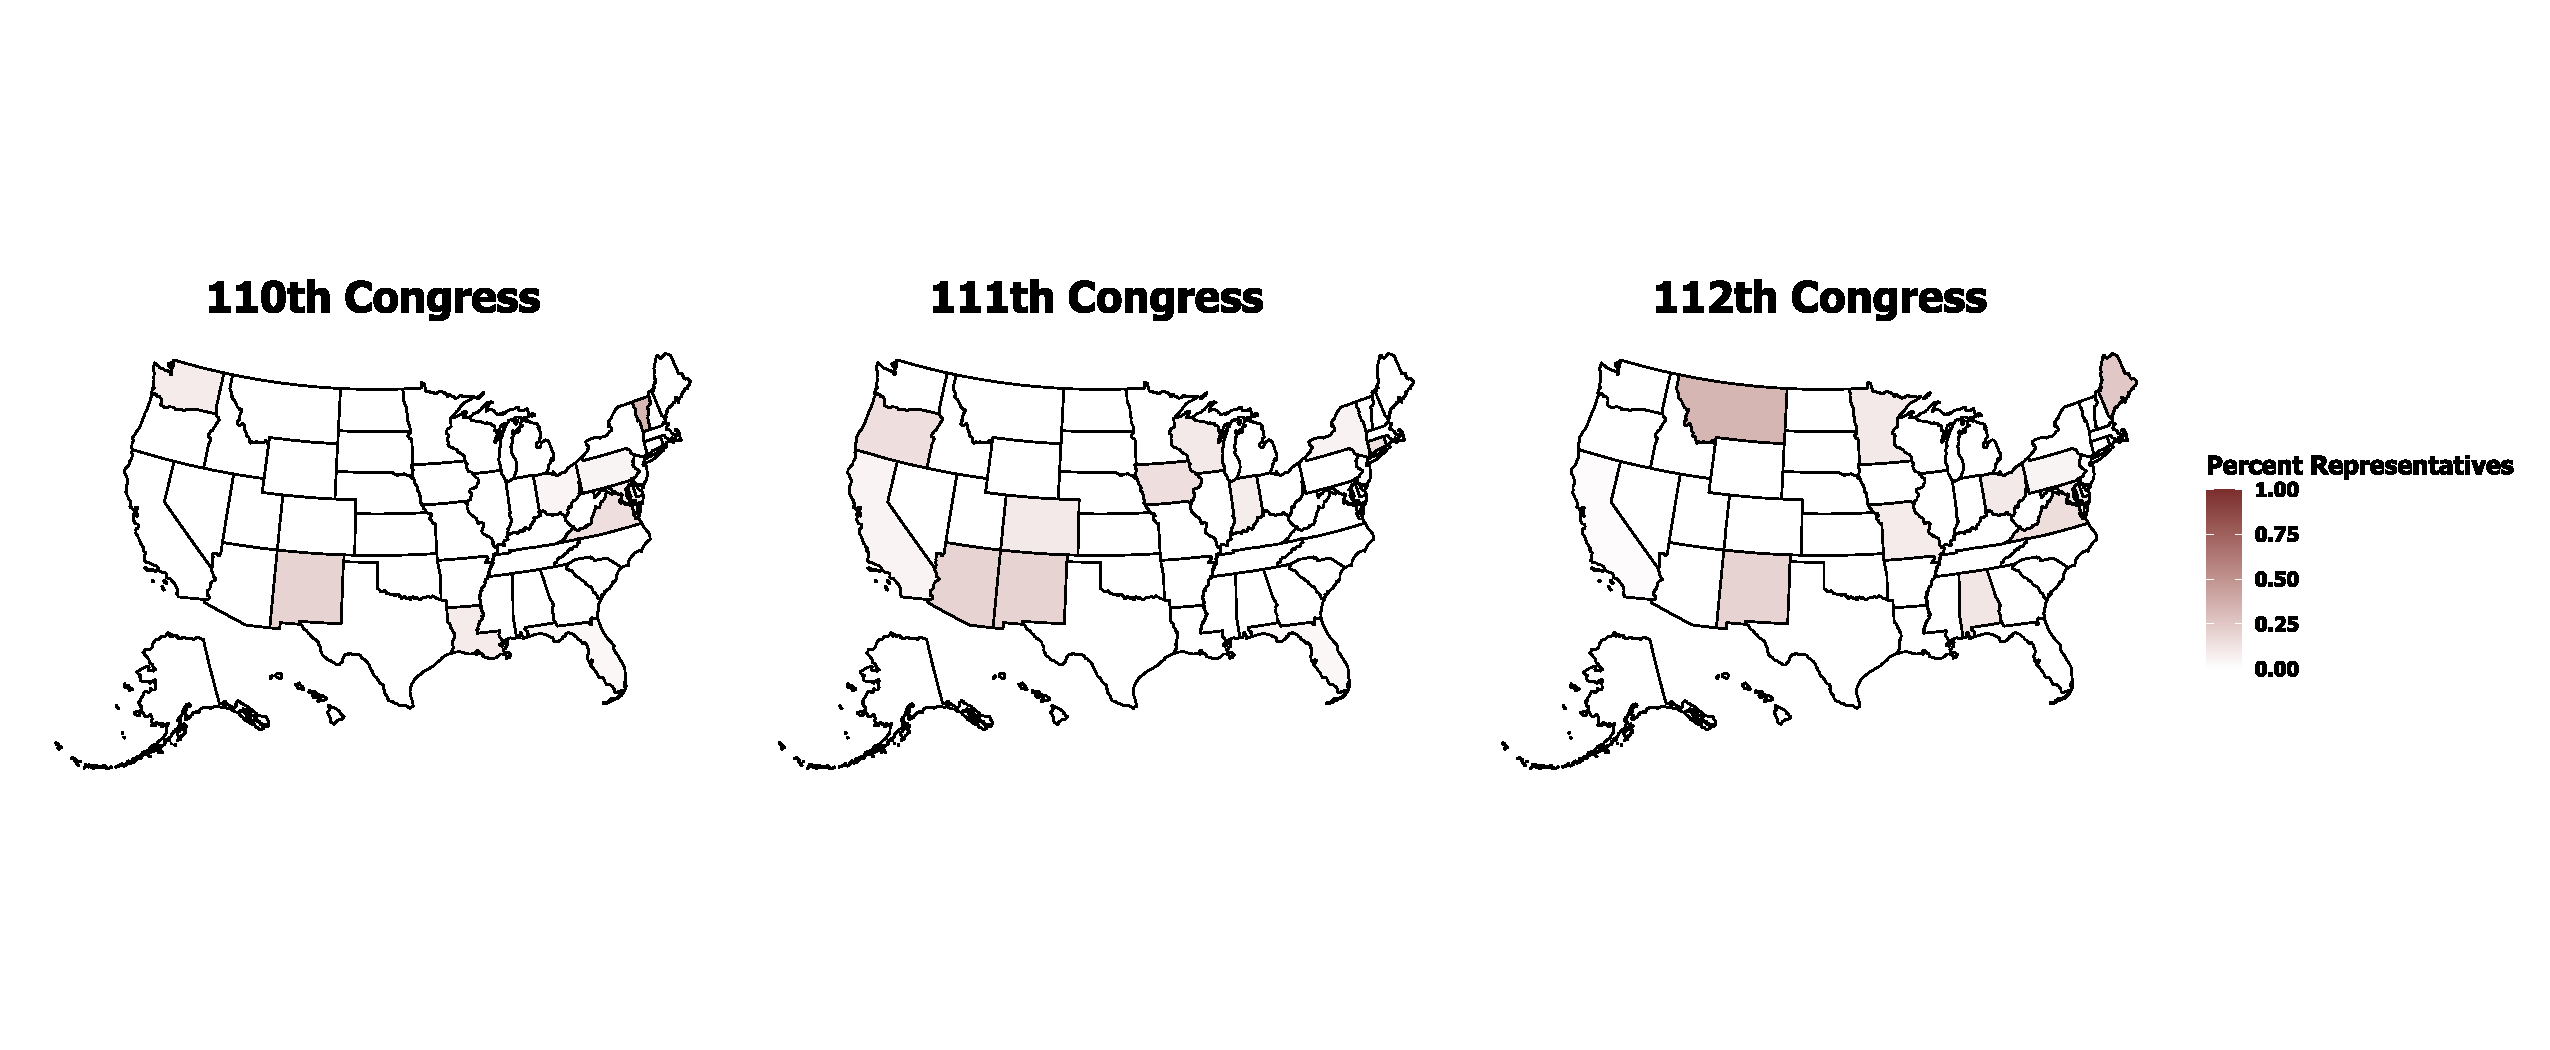
\includegraphics[width=1\textwidth]{womens_SVU_maps.pdf}
		\begin{minipage}{0.92\textwidth}
			\smallskip
			\small
			\textit{Note:}  Plots indicate proportion of legislators contacting federal agencies on behalf of women (excluding casework) at least once per congressional term for the 110th, 111th, and 112th Congresses. Darker shades of red indicate higher values.
		\end{minipage}
	\end{figure}
	
	\begin{figure}[h!]
		\caption*{\textbf{Figure 3.3: Substantive Representation of Racial/Ethnic Minorities Over Time}}\label{fig3.3}
		\centering
		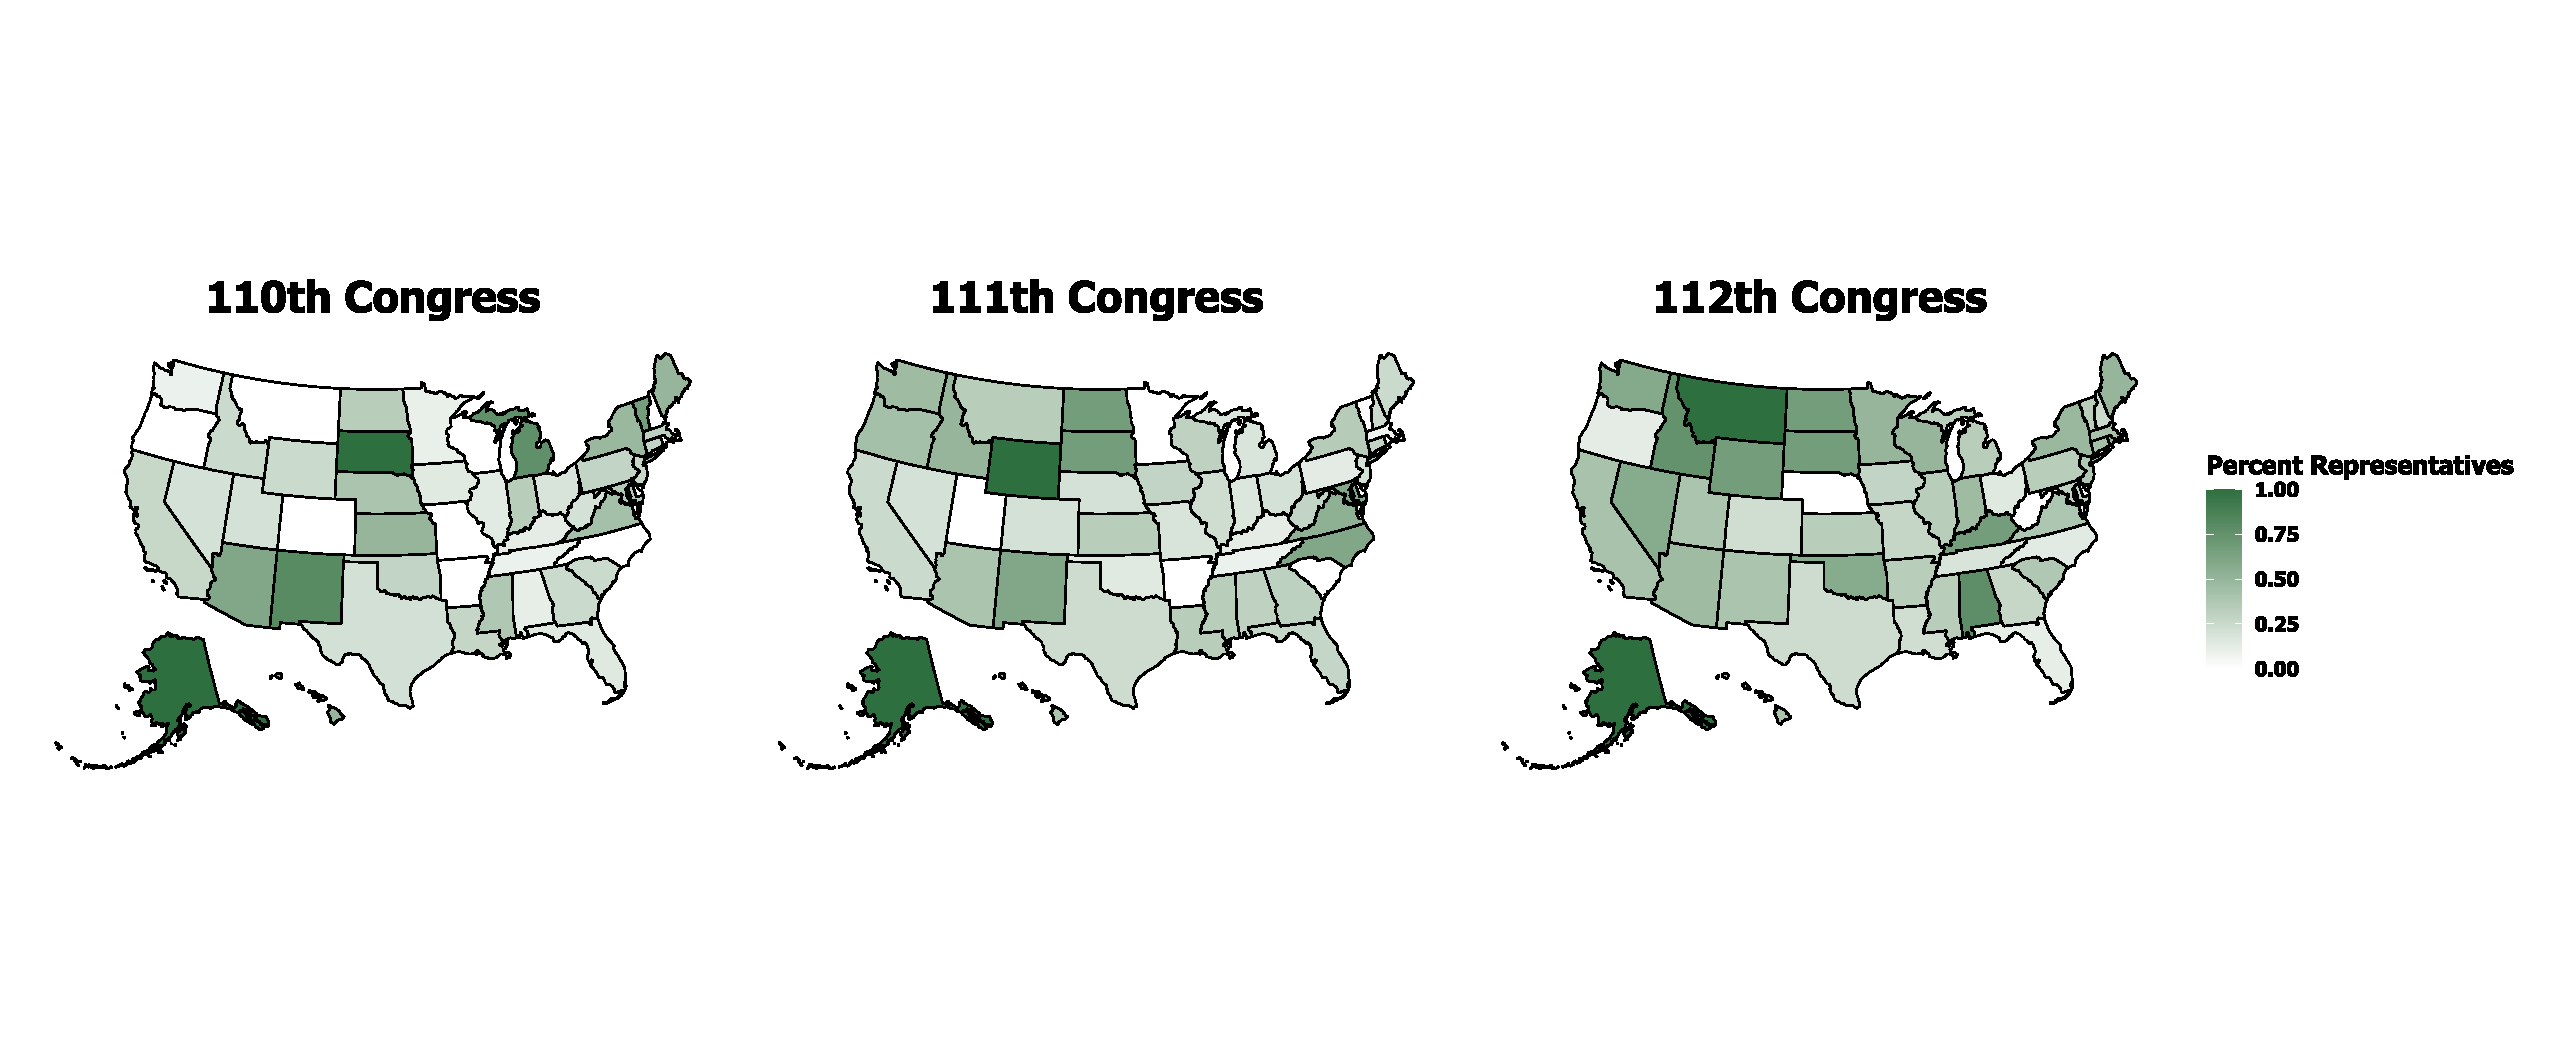
\includegraphics[width=1\textwidth]{minority_SVU_maps.pdf}
		\begin{minipage}{0.92\textwidth}
			\smallskip
			\small
			\textit{Note:} Plots indicate proportion of legislators contacting federal agencies on behalf of racial or ethnic minorities (excluding casework) at least once per congressional term for the 110th, 111th, and 112th Congresses. Darker shades of green indicate higher values.
		\end{minipage}
	\end{figure}
	
	\newpage
	
	Open AI's Chat GPT \parencite{openai_chatgpt} supported me in debugging for this project as well as compiling sources cited into a neat bibliography (APA 7th Edition). I used \texttt{R} packages \texttt{usmap, ggfortify, cem, MASS, stargazer, xtable, purrr, doMC, doRNG, tidyverse, ggplot2, ggtext, showtext, systemfonts, patchwork, foreach} and their dependencies in data analysis and synthesis of plots.\\
	
		\printbibliography 
		
\end{document}
